\documentclass[10pt]{article}
\usepackage{icmlko}

\icmlmeta{IP 파운데이션 월드모델}{259}{자리가 아니라 길이다}{잡음 여덟 개는 안 밀어내는데 진짜 축 둘은 밀어낸다 --- 나무의 길이 바뀌는 것이었다}

\begin{document}

\twocolumn[
\icmlheader

\begin{abstract}
노트 258은 도메인 전용 축을 쌓을수록 웹툰이 낸다는 것을 쟀고(제 축 $+$0.021,
남의 축 $-$0.028), 원인을 ``\textbf{자리 예산}''으로 짐작했다 --- 열이 늘면
나무의 분할 예산과 능형의 벌점 예산을 나눠 쓴다는 것. 그럴듯했다. \textbf{틀렸다.}
값싼 검정이 있다: \emph{잡음} 열로 같은 자리를 먹여 보면 된다. 모바일에만
값이 있는 난수 열을 둘 · 넷 · 여덟 개 넣었다. 웹툰이 $+$0.0003 · $-$0.0013 ·
$-$0.0046 이다. \textbf{여덟 개를 넣어도 진짜 축 둘($-$0.0205)의 4분의 1 도
안 된다.} 자리 문제가 아니다. 그러면 무엇인가. 형식별로 갈랐더니
\textbf{나무가 낸다} --- F18 $-$0.0286($t{=}-5.83$) 대 F21 $-$0.0067
($t{=}-2.48$). 둘을 합치면 답이 나온다: \textbf{나무는 잡음 열을 안 쓰고
지나가지만, 쓸모 있는 열은 위쪽에서 갈라 버린다.} 그 갈래가 아홉 도메인이
같이 쓰는 길이라, 모바일에 좋은 분기가 생기면 웹툰 행이 다른 길로 간다.
비어 있는 방이 좁아진 게 아니라 \textbf{길이 다시 놓인 것}이다. 겸사겸사
규약도 확인했다. 모바일 성분 3 하나만 넣으면 판이 0.4703 으로 지금(0.4687)보다
높은데, \textbf{그걸 고르는 것은 유보를 보고 고르는 것}이다. 대신 규약
자체를 견줬다 --- ``통과한 것 전부'' 대 ``제일 센 것 하나''를 세 도메인에
똑같이 적용하니 전자가 두 짝에서 다 이긴다(0.4687 대 0.4628 · 0.4678 대
0.4642). \textbf{규약이 그대로 서고, 노트 258의 모바일 거부도 그대로 선다.}
\end{abstract}
]

\section{자리 짐작을 검정으로 바꿨다}

노트 258의 마지막 줄은 짐작이었다.

\begin{quote}\small
값은 전용이라 서로 안 보지만 \textbf{모형은 하나}이고, 열이 늘면 나무의
분할 예산과 능형의 벌점 예산을 나눠 쓴다. 웹툰이 기대던 손 축 다섯의 자리가
좁아진다.
\end{quote}

짐작인 채로 남겨 두면 안 되는 종류다 --- 맞으면 처방이 명확하기 때문이다
(예산을 키운다). 검정이 값싸다. \textbf{자리만 먹고 정보는 안 주는 열}을
넣어 보면 된다.

\begin{figure}[t]
\centering

\includegraphics[width=\columnwidth]{figs/noise.pdf}
\caption{왼쪽 --- 잡음 열은 몇 개를 넣어도 웹툰을 거의 안 건드린다.
오른쪽 --- 진짜 축 둘의 손해가 어느 형식에서 나나.}
\end{figure}

\begin{center}\small
\begin{tabular}{lrr}
\hline
넣은 것 & 웹툰 차 & $t$ \\
\hline
\textbf{모바일 진짜 축 2개} & $\mathbf{-0.0205}$ & $-$6.23 \\
잡음 2개 (모바일) & $+$0.0003 & 0.16 \\
잡음 2개 (게임) & $-$0.0027 & $-$1.91 \\
잡음 4개 (모바일) & $-$0.0013 & $-$0.49 \\
잡음 8개 (모바일) & $-$0.0046 & $-$1.59 \\
\hline
\end{tabular}
\end{center}

\textbf{잡음 여덟 개가 진짜 둘의 4분의 1 도 안 된다.} 열 개수가 원인이라면
여덟이 둘보다 네 배 나빠야 한다. 자리 짐작은 반증됐다.

\section{나무가 낸다}

형식별로 웹툰의 손해를 갈랐다.

\begin{center}\small
\begin{tabular}{lrrr}
\hline
형식 & 웹툰 차 & 짝 SE & $t$ \\
\hline
F21 능형 & $-$0.0067 & 0.0027 & $-$2.48 \\
\textbf{F18 나무} & $\mathbf{-0.0286}$ & 0.0049 & $\mathbf{-5.83}$ \\
F23 판 & $-$0.0205 & 0.0033 & $-$6.22 \\
\hline
\end{tabular}
\end{center}

능형도 조금 내지만 나무가 네 배 넘게 낸다.

두 결과를 합치면 기전이 하나로 좁혀진다.

\begin{quote}
나무는 \textbf{쓸모없는 열을 안 쓰고 지나간다} --- 그래서 잡음 여덟 개가
아무 일도 안 한다. 그런데 \textbf{쓸모 있는 열은 위쪽에서 갈라 버린다.}
그 분기는 아홉 도메인이 함께 내려가는 길이다. 모바일 행을 잘 가르는 분기가
뿌리 근처에 생기면 \textbf{웹툰 행도 그 분기를 지나} 다른 잎으로 간다.
\end{quote}

노트 258이 ``자리가 좁아진다''고 이름 붙였는데, 좁아진 것이 아니라
\textbf{길이 다시 놓인 것}이다. 방이 좁아진 게 아니라 복도가 옮겨졌다.

이것은 노트 251이 ``나무는 계수가 없고 문턱을 나눠 쓴다''고 적은 것의
자연스러운 귀결이고, 노트 242가 ``나무는 어긋나는 4\%를 문턱으로 쓴다''고
적은 것의 대가다. 나무의 강점과 약점이 같은 성질에서 나온다.

\paragraph{처방이 달라진다} 자리 문제였다면 나무를 깊게 하거나 잎을 늘리면
됐다. 길 문제면 그것으로는 안 된다 --- 깊게 해도 뿌리 근처 분기는 그대로다.
필요한 것은 \textbf{도메인마다 다른 길}인데, 그것은 노트 241이 이미 재고
거부한 물건이다(도메인별 유연성은 넷에서 손해).

\section{규약을 견줬다, 축을 고르지 않고}

갈라 보다가 눈에 걸린 것이 있다. 모바일 성분을 하나씩 넣어 보면

\begin{center}\small
\begin{tabular}{lrrr}
\hline
 & 판 & 모바일 & 웹툰 \\
\hline
성분 2 만 & 0.4664 & $+$0.0037 ($t{=}0.4$) & $-$0.0107 \\
\textbf{성분 3 만} & \textbf{0.4703} & $+$0.0379 ($t{=}2.2$) & $-$0.0162 \\
둘 다 & 0.4678 & $+$0.0375 & $-$0.0205 \\
\hline
\end{tabular}
\end{center}

\textbf{성분 3 하나만 넣으면 0.4703 으로 지금(0.4687)보다 높다.} 성분 2 는
모바일에 아무것도 못 주면서($t{=}0.4$) 웹툰만 깎는다.

여기서 성분 3 만 고르고 싶어진다. \textbf{그러면 안 된다} --- 둘 다 학습
구간 검사를 통과했고, 둘 중 하나를 고르는 근거는 오직 유보 수뿐이다.
노트 216 · 224 · 234 · 241에서 거부한 것과 정확히 같은 자리다.

대신 물음을 \emph{규약} 수준으로 올렸다. ``통과한 것을 전부 쓴다''와
``제일 센 것 하나만 쓴다''를 \textbf{세 도메인에 똑같이} 적용해 견준다.
이것은 도메인별 선택이 아니라 하나의 설계 결정이다.

\begin{figure}[t]
\centering
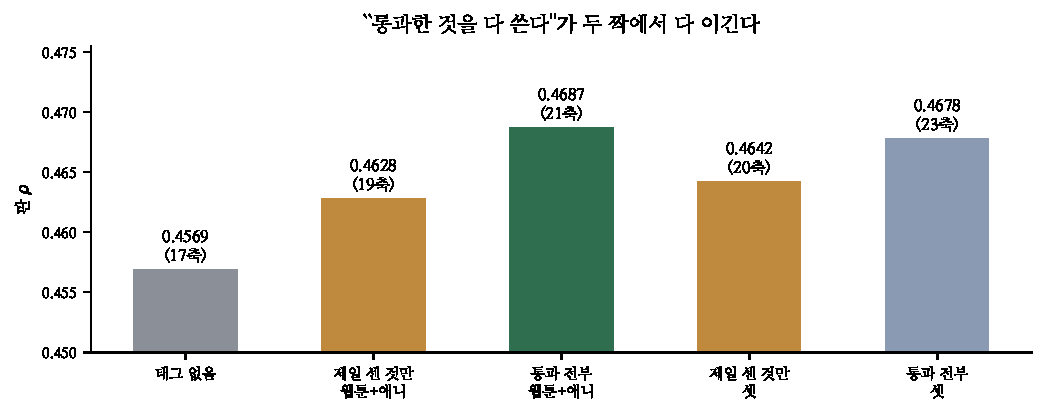
\includegraphics[width=\columnwidth]{figs/rule.pdf}
\caption{규약 둘을 두 짝(웹툰$+$애니, 셋)에 각각 적용.}
\end{figure}

\begin{center}\small
\begin{tabular}{lrr}
\hline
규약 & 축 & 판 \\
\hline
태그 없음 & 17 & 0.4569 \\
제일 센 것만 · 웹툰$+$애니 & 19 & 0.4628 \\
\textbf{통과 전부 · 웹툰$+$애니} & 21 & \textbf{0.4687} \\
제일 센 것만 · 셋 & 20 & 0.4642 \\
통과 전부 · 셋 & 23 & 0.4678 \\
\hline
\end{tabular}
\end{center}

\textbf{``통과한 것 전부''가 두 짝에서 다 이긴다}(0.4687 대 0.4628 ·
0.4678 대 0.4642). 규약이 그대로 서고, 그 규약 아래에서 노트 258의
\textbf{모바일 거부도 그대로 선다}(23축 0.4678 $<$ 21축 0.4687).

\section{남은 자리}

판은 0.4687, 축 스물하나 그대로다. 이 노트는 판을 안 움직였지만 짐작 하나를
지웠다 --- \textbf{자리를 늘리는 처방은 없다.} 노트 258의 ``남은 것'' 첫
줄(``나무 깊이 · 능형 알파를 축 수에 맞춰 늘리면?'')이 닫혔다.

\paragraph{남은 것}
\begin{center}\small
\begin{tabular}{ll}
\hline
갈래 & 왜 \\
\hline
21축 천장 & 노트 252의 CV 천장은 17축 것이다. 다시 재야 한다 \\
길 문제 & 도메인별 길은 노트 241이 거부했다. 다른 형태가 있나 \\
성분 2 같은 것 & 제 도메인에 안 주면서 남만 깎는 축을 미리 아나 \\
게임 259건 & 조각 검사가 못 돈다 \\
\hline
\end{tabular}
\end{center}

\paragraph{규약} ``자리가 모자라서''라고 쓰기 전에 \textbf{잡음으로 같은
자리를 먹여 본다.} 잡음이 안 밀어내면 자리 문제가 아니다. 노트 253의
``덜어 내 본다''와 같은 종류의 한 줄짜리 검정이고, 이번에도 짐작을 지웠다.

\end{document}
